\part*{Modelo Conceptual}

\section{Formulación del problema}

El presente Trabajo Práctico busca representar la estrategia comercial de una consultora de software (\textit{software factory}). En cuanto a la selección de proyectos, se busca 
la mejor combinación entre aprovechar el trabajo de los programadores y mantener cierta reserva de capacidad para no tener que rechazar proyectos \textit{atractivos}, es decir,
de mayor rentabilidad.\\

La simulación se basó en datos ``pseudo-reales'', dada la dificultad que implicaba la recolección de datos y la escasez de ellos.\\

\section{Modelado del problema}

Se definieron las siguientes entidades:

\begin{itemize*}
    \item Proyecto
    \item Organización
    \item \textit{Workflow}
\end{itemize*}

Los proyectos fueron modelados como una \textit{tupla} de horas-hombre, precio por hora, desarrolladores pretendidos, desarroladores extra y fecha de entrega. Estas propiedades describen el tamaño, el ingreso que representa, la cantidad de desarrolladores que fueron negociados, los desarrolladores que fueron agregados al proyecto para cumplir la fecha y el
tiempo máximo de desarrollo, respectivamente.\\

La organización representa la software factory en sí misma, y fue modelada como una entidad que posee un conjunto de desarrolladores, un \textit{workflow}, una cola donde 
llegan los nuevos proyectos y una estrategia de aceptación de proyectos.\\

La entidad \textit{workflow} está constituida por el conjunto de proyectos en desarrollo y la estrategia de asignación de recursos.\\

\subsection{Restricciones - Límites del problema}

Para el modelado del problema, se ignoraron algunas variables reales del problema, que hubieran hecho impracticable la representación y resolución del mismo. El simulador se ve 
restringido a un uso académico, dado que no tiene en cuenta muchas variables del mundo real.

Las variables que se ignoran son: \\

\begin{itemize}
    \item La capacitación del personal y su curva de aprendizaje: se supone que el programador conoce el proyecto y no tarda en empezar a programar.
    \item Nuevos requerimientos en el proyecto: Desde un primer momento, se conoce el tiempo de desarrollo que involucrará un proyecto, no se pueden agregar 
            funcionalidades a la mitad del desarrollo.
    \item Competencia, mercado, precios: estas variables están sujetas a la llegada de proyectos, pero no se toman como variables separadas sino que se engloban en la 
        llegada de proyectos.
    \item La situación financiera de la empresa: se considera que la empresa tiene fondos como para pagar sus costos de funcionamiento durante la duración de la simulación.
    \item El traspaso de desarrolladores: se supone que la cantidad de desarrolladores permanece constante a lo largo de la simulación.
\end{itemize}

\subsection{Variables de control}
Se definen como variables de control del problema, las siguientes:

\begin{itemize}
    \item Cantidad de programadores que se ``reservan'' (para proyectos \textit{atractivos}).
    \item Estrategia de aceptación de proyectos.
\end{itemize}

\section{Variables aleatorias}
Se encontraron las siguientes variables aleatorias:

\begin{itemize}
    \item Cantidad de proyectos que llegan en un determinado período.
    \item Tipo del proyecto (pequeño, mediano o grande).
    \item Tamaño del proyecto (medido en horas-hombre).
    \item Precio por hora del proyecto.
    \item Cantidad de desarrolladores pretendidos. Se considera que a la hora de negociar el proyecto, se acuerda un numero pretendido de desarrolladores asignados al proyecto.
\end{itemize}

\section{Funciones objectivo}
Las funciones objectivo que se consideran son:

\begin{itemize}
    \item Costo de oportunidad, ingreso que hubieran generado los proyectos rechazados.
    \item Ingreso generado por los proyectos aceptados.
    \item Porcentaje de recursos utilizados.
\end{itemize}

Para representar los resultados y la evolución de estas magnitudes, se tiene una vista que muestra, paso por paso, estos valores y, al final de la simulación, un
gráfico con los intervalos de valores. \\

Cabe destacar que para esto, previamente se debe debe fijar, para las estrategias de decisión que los tengan, los parámetros de entrada, buscando que sean los
que arrojen los mejores resultados.\\

\section{Plan de cuadros}

El diagrama de cuadros, que se utilizará para llevar a cabo la simulación será el siguiente

\begin{table}[H]
\begin{center}
 \begin{tabular}{|c|c|c|c|c|}
  \hline
  \multirow{2}{*}{\textbf{Estrategia}} & \multirow{2}{*}{\textbf{Devs Reservados}} & \textbf{Ingreso} & \textbf{Costo de Oportunidad} & \textbf{\% Recursos utilizados} \\
                                       &                                         &$[min, mean, max]$ & $[min, mean, max]$          & $[min, mean, max]$ \\
  \hline
  \hline
  \multirow{3}{*}{Estrategia 1} & 0 &  $[... , ... ,...]$ & $[... , ... ,...]$ & $[... , ... ,...]$\\
                                & 2 & $[... , ... ,...]$ & $[... , ... ,...]$ & $[... , ... ,...]$\\
                                & 4 & $[... , ... ,...]$ & $[... , ... ,...]$ & $[... , ... ,...]$\\
                                & 6 & $[... , ... ,...]$ & $[... , ... ,...]$ & $[... , ... ,...]$\\
  \hline
  \multirow{3}{*}{Estrategia 2} & 0 &  $[... , ... ,...]$ & $[... , ... ,...]$ & $[... , ... ,...]$\\
                                & 2 & $[... , ... ,...]$ & $[... , ... ,...]$ & $[... , ... ,...]$\\
                                & 4 & $[... , ... ,...]$ & $[... , ... ,...]$ & $[... , ... ,...]$\\
                                & 6 & $[... , ... ,...]$ & $[... , ... ,...]$ & $[... , ... ,...]$\\
  \hline
 \end{tabular}
 \caption{Plan de cuadros para la simulación}
\end{center}
\end{table}

\section{Diagrama de Bloques}

\begin{figure}[H]
\begin{center}
 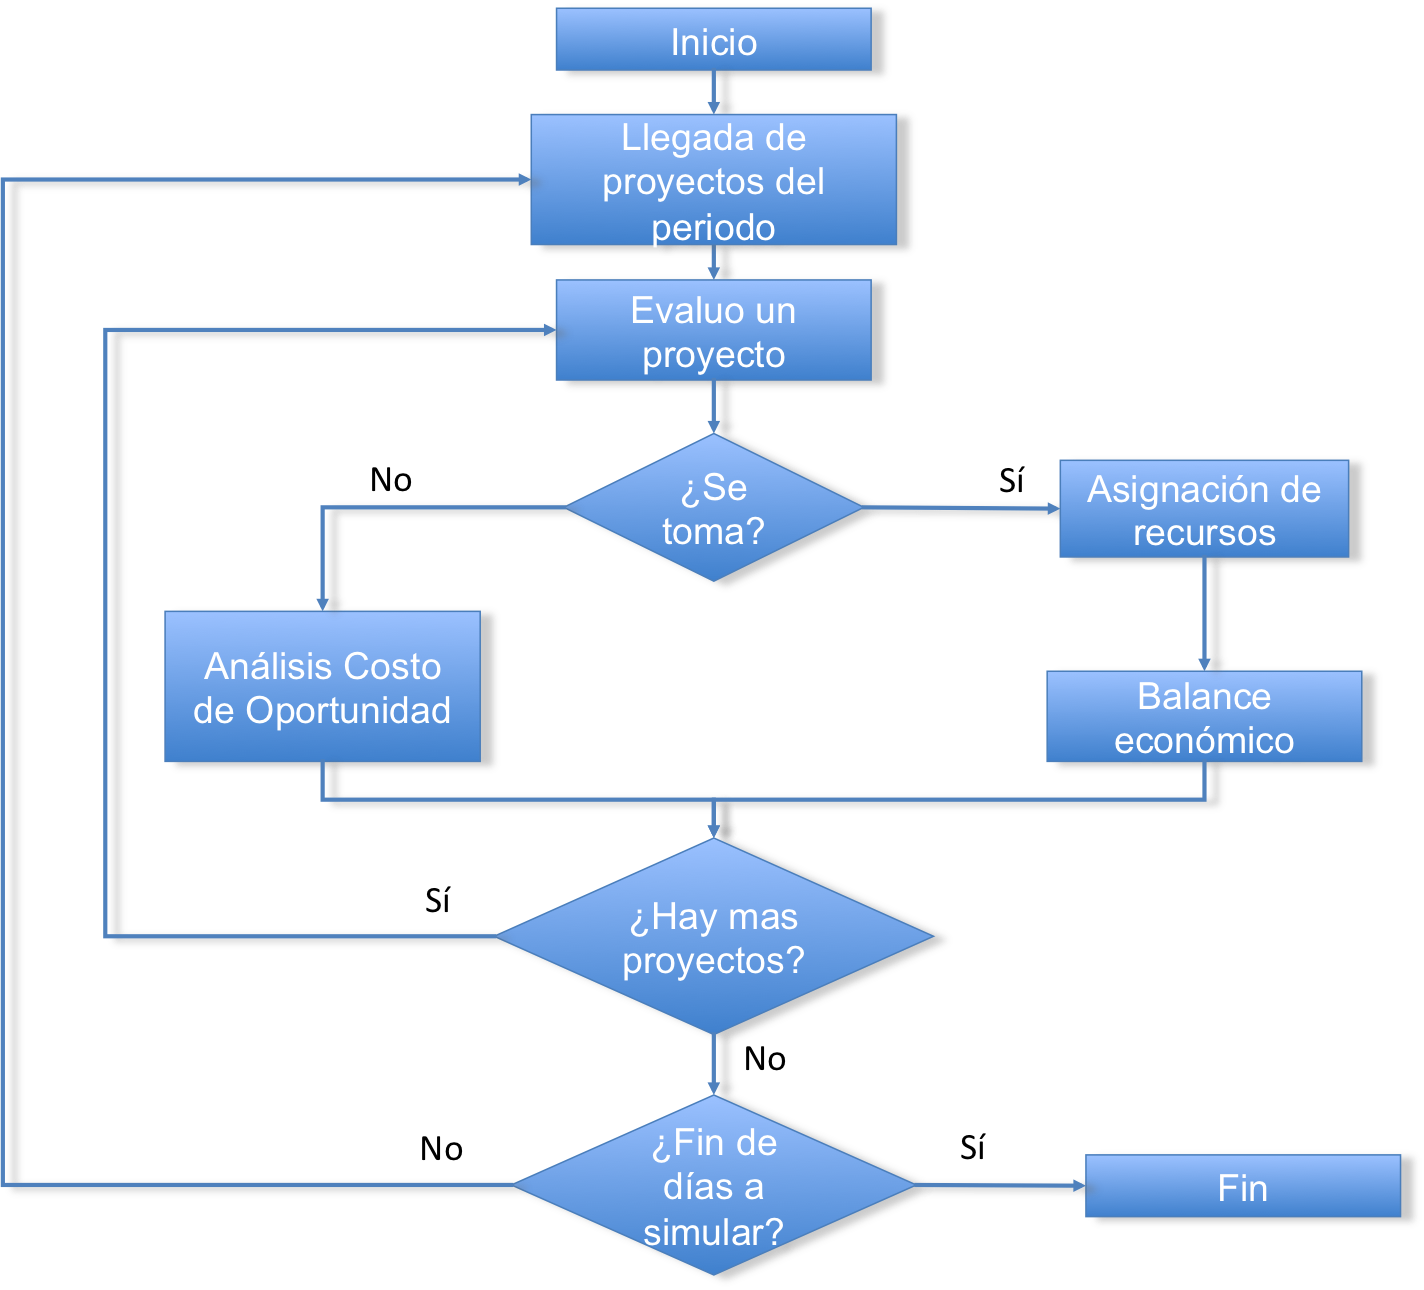
\includegraphics[width=\textwidth,height=\textheight,keepaspectratio]{./images/bloques.png}
 % bloques.png: 1424x1290 pixel, 150dpi, 24.11x21.84 cm, bb=0 0 683 619
\end{center}

\caption{Diagrama de bloque del simulador}
\label{fig:bloque}
\end{figure}


\section{Diagrama de Flujo}

\begin{multicols}{2}
Muestras artificiales (MA)\\
Variables

\begin{enumerate*}
    \item Cantidad de Proyectos por mes(CA)\\
            VA Poisson ($\lambda$)
    \item Tipo de Proyecto (TP)\\
            VA Uniforme
    \item Tamaño de Proyecto [hs]\\
            VA Triangular(a, b, c)
    \item Costo Hora-Hombre [\$]\\
            VA Triangular(a, b, c)
    \item Desarrolladores pretendidos [hombres]\\
            VA Triangular(a, b, c)
\end{enumerate*}
\vfill
\columnbreak
\begin{itemize*}
 \item T: Tiempo del reloj de la simulación
 \item Tmax: Cantidad de tiempo a simular
 \item P: Proyecto actual
 \item R: Recursos (programadores)
 \item M: Dinero
 \item CO: Costo de Oportunidad
 \item M(P): Ganancia del proyecto P
 \item R(P): Función de asignación de recursos usados por el proyecto P
 \item D(P): Decide si un proyecto es entregable en plazo considerando los proyectos que ya se tomaron
 \item O(P\_1, ..., P\_n): Ordena los proyectos P\_1 a P\_n según el criterio de la estrategia y marca al resultante P\_1 como atractivo
 \item A(P): Si la estrategia considera el proyecto atractivo
 \item E(P): Desarrolladores reservados asignados al proyecto

\end{itemize*}

\end{multicols}

\begin{figure}[H]
\begin{center}
 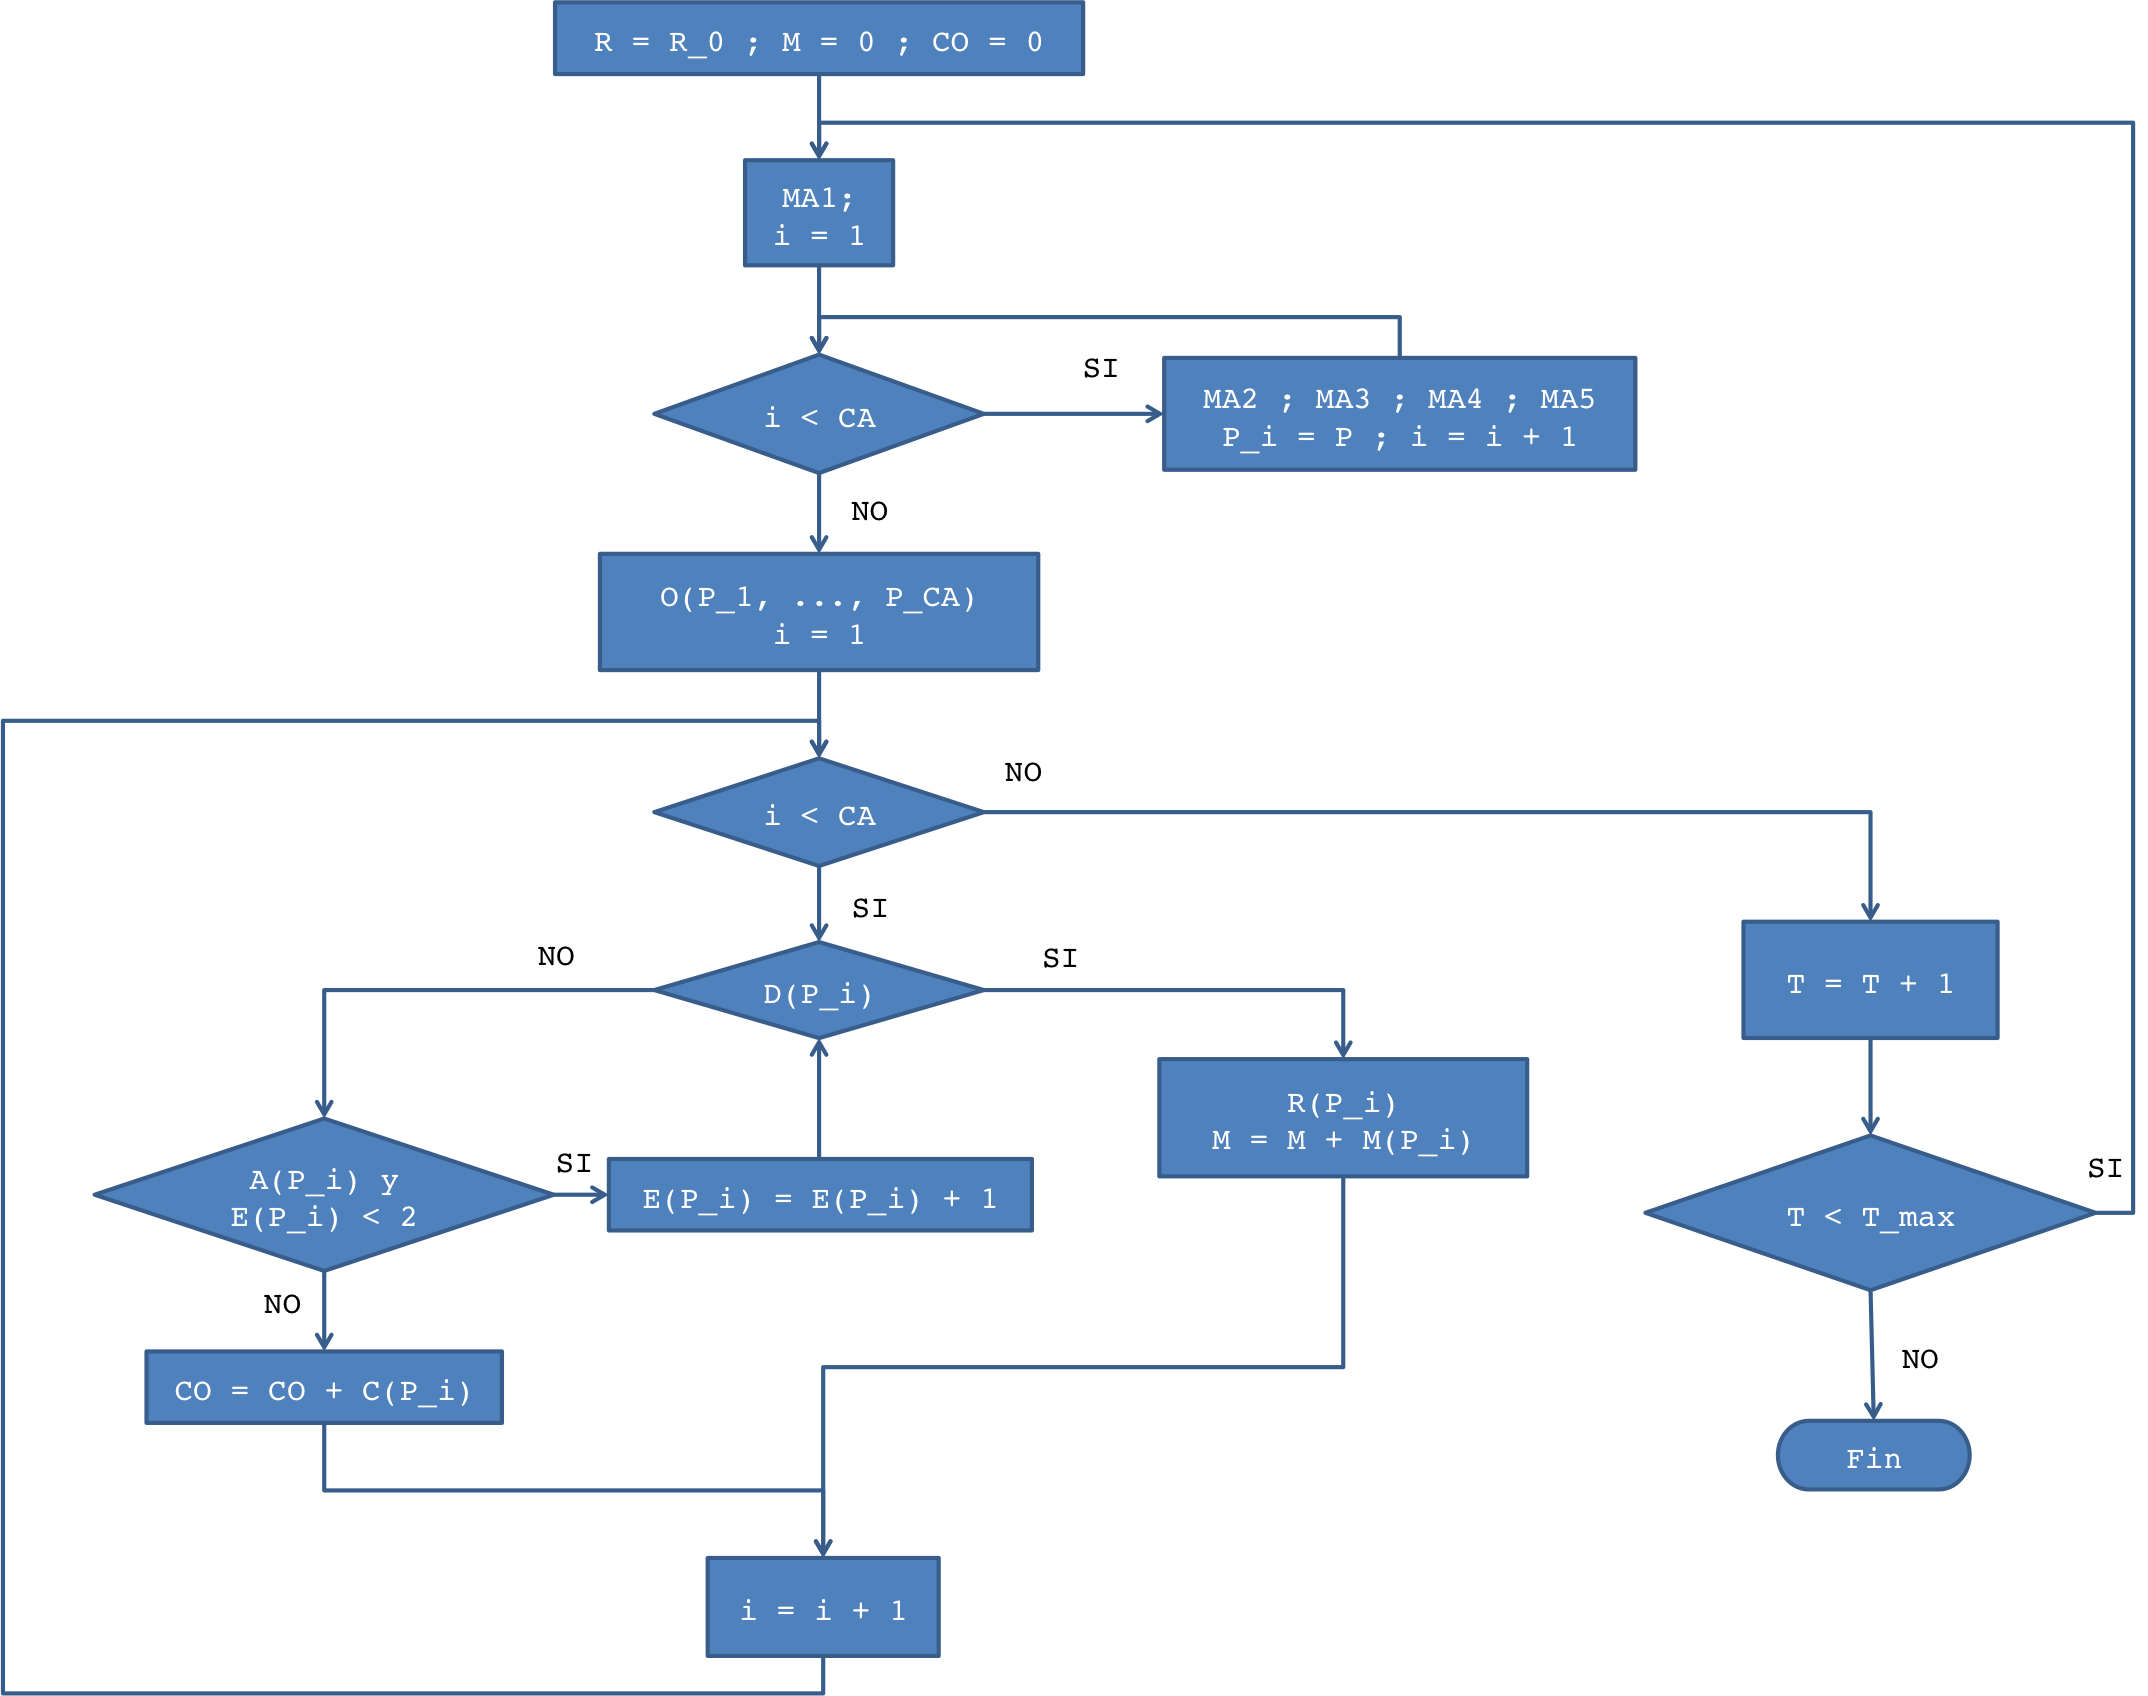
\includegraphics[width=\textwidth,height=\textheight,keepaspectratio]{./images/flujo.png}
\end{center}

\caption{Diagrama de flujo del simulador}
\label{fig:flujo}
\end{figure}

\section{Plazo de entrega}
Al momento de recibir un proyecto nuevo, se tiene la cantidad de horas hombre que este requiere y la cantidad de desarrolladores pretendidos para el proyecto. 
A partir de estas 2 variables se obtiene el plazo en meses del proyecto, haciendo el cociente entre las horas hombre y la cantidad de horas por mes que trabajarian 
los desarrolladores pretendidos.


\section{Estrategias de decisión}

Tanto en el diagrama de bloques como en el diagrama de flujo se observa una función o estrategia de decisión para aceptar o no un proyecto. A continuación se detallan 
las estrategias que se estudiarán. Debe ser tomado en cuenta que independientemente de la estrategia, si no se tienen suficientes recursos como para completar el proyecto 
antes de su fecha de entrega el valor de $D(P)$, es decir la función que acepta o no el proyecto, es siempre $NO$.

\begin{enumerate}
    \item Se ordenan los proyectos arribados según el precio por hora, luego por la cantidad de horas del proyecto, y se aceptan, en caso de ser posible su desarrollo, en ese orden.\\

    \item Se ordenan los proyectos encolados según su facturación (precio por hora * horas-hombre), luego por el precio por hora, y se aceptan, en caso de ser posible, en ese orden.\\
\end{enumerate}



\section{Estrategia de asignación de recursos}

Para la asignación de recursos, al comienzo de cada período, se calcula la cantidad de horas/hombre que se van a asignar al proyecto de la siguiente manera: \\
se toma el total de horas/hombre restantes del proyecto, llamémosle $W$, y se lo divide por la 
cantidad de períodos que faltan hasta la fecha entrega. Esto es la cantidad de horas que se le asignarán a ese proyecto en este período.
En caso de queden recursos sin asignar, se asignarán al proyecto más cercano a su fecha de entrega. 
De esta forma, se busca balancear la asignación de recursos, buscando cumplir con las fechas de entrega, y en caso de ser posible, adelantar los proyectos 
cercanos a su fin, con el objetivo de liberar recursos para poder aceptar otros nuevos.
